\chapter{Sesgos en Aprendizaje Autom\'atico}\label{chapter:state-of-the-art}

% - Justicia / Sesgos / Equidad ok
% - Casos Controversiales. ok
% - Fuentes de Sesgos ok
% - (Definiciones / Algoritmos) para tratar los sesgos ok
% - Datasets Recursos de sesgos ok
% - Discusi'on ok

% Los algoritmos de aprendizaje autom\'atico est\'an presentes en casi todos los aspectos de la vida moderna,
% desde proporcionar recomendaciones de pel\'iculas y facilitar compras en l\'inea hasta influir en b\'usquedas en la web
% y sugerir conexiones emocionales con otras personas. Este fen\'omeno se extiende incluso a escenarios m\'as riesgosos,
% como el diagn\'ostico y tratamiento m\'edico, donde el uso de estos algoritmos ha experimentado un notable aumento.
% La versatilidad de estas herramientas abarca diversas \'areas, como la optimizaci\'on de procesos empresariales, la 
% mejora de la eficiencia de los sistemas de transporte \parencite{autonomous_driving}, y la personalizaci\'on de servicios en 
% sectores como el financiero y el comercio.

% A medida que estos algoritmos se aplican con mayor frecuencia en \'ambitos m\'as cr\'iticos, como
% pr\'estamos bancarios \parencite{fairness_def}, evaluaci\'on de riesgos de salud, contrataci\'on, evaluaci\'on de desempe\~no laboral y
% justicia penal \parencite{compas}, se genera una creciente preocupaci\'on acerca de su capacidad para mantener de manera involuntaria 
% sesgos sociales y prejuicios hist\'oricos.
% Este cap\'itulo proporciona una base te\'orica s\'olida para los desaf\'ios que enfrentan los modelos de aprendizaje autom\'atico en t\'erminos
% de sesgos e injusticias. Para ello, se discute la presencia de sesgos en sistemas que utilizan modelos de aprendizaje autom\'atico, como 
% el sistema COMPAS y los datos de la Encuesta de Gastos M\'edicos. Se presentan diversas fuentes y tipos de sesgos
Este cap\'itulo presenta una revisi\'on del estado del arte sobre la problem\'atica de la justicia y la equidad en los modelos de 
aprendizaje autom\'atico. Se discuten conceptos clave como la existencia de sistemas algor\'itmicos sesgados, las principales fuentes
y tipos de sesgos, as\'i como las definiciones predominantes de equidad y t\'ecnicas para la detecci\'on y mitigaci\'on de sesgos.
Adem\'as, se hace especial \'enfasis en el papel que juegan los \emph{datasets} con atributos protegidos anotados en el desarrollo
y evaluaci\'on de t\'ecnicas para promover la justicia algor\'itmica. Por \'ultimo, el cap\'itulo presenta un an\'alisis de los 
principales \emph{datasets} utilizados en la literatura para el tratamiento de sesgos.

\section{Sistemas Sesgados}

    La presencia de sesgos en sistemas que utilizan modelos de aprendizaje autom\'atico es un tema cr\'itico que ha sido
    ampliamente estudiado en los \'ultimos a\~nos. 
    
    En el \'ambito de la justicia penal, el caso m\'as conocido es el de COMPAS~\parencite{propublica}
    (en ingl\'es \emph{Correctional Offender Management Profiling for Alternative Sanctions}). Este sistema es un algoritmo de predicci\'on
    de riesgo de reincidencia criminal, que se ha utilizado en las cortes de Estados Unidos para ayudar a los jueces a determinar la 
    probabilidad de que una persona reincurra en un delito. Se demostr\'o que el software estaba sesgado hacia las personas 
    afroamericanas, o sea, dados dos individuos con el mismo perfil criminal, solo basta que uno sea afroamericano para que el
    sistema prediga que tiene una mayor probabilidad de reincidir respecto al que no lo es. En un estudio, se determin\'o que, 
    en comparaci\'on con la evaluaci\'on realizada por personas no expertas, el desempe\~no del sistema no demostr\'o mejoras 
    significativas~\parencite{compas2}. 
    
    Los datos de la Encuesta de Gastos M\'edicos (MEPS\footnote{\url{https://meps.ahrq.gov/mepsweb/about_meps/spanish.jsp}}, 
    por sus siglas en ingl\'es) son una colecci\'on de encuestas representativas a nivel nacional, de acceso p\'ublico, que proporcionan 
    datos sobre el uso y los costos de los servicios de atenci\'on m\'edica para la poblaci\'on civil no institucionalizada de los Estados Unidos. 
    Es com\'un el empleo de estos datos para el desarrollo de modelos predictivos de gastos de salud, con el objetivo de guiar decisiones 
    en la gesti\'on de la atenci\'on m\'edica, enfermedades y costos asociados. Se ha comprobado que estos modelos tambi\'en capturan sesgos, 
    generando un sesgo significativo en perjuicio de las personas afroamericanas. Concretamente, existe una menor probabilidad de que 
    las personas afroamericanas sean identificadas como pacientes con altos gastos futuros en comparaci\'on con las personas personas blancas, 
    lo que resulta en una menor probabilidad de recibir gesti\'on de atenci\'on~\parencite{understanding}.

    Los sesgos presentes en la sociedad tambi\'en se han identificado en anuncios generados por modelos de aprendizaje 
    autom\'atico~\parencite{sweeney2013discrimination,datta2015automated} y en motores de b\'usqueda web~\parencite{unequal_rep}, 
    pricipalmente en relaci\'on al g\'enero. Adem\'as, se han detectado sesgos en otros sistemas como los 
    chatbots~\parencite{chatbot_bias}, as\'i como en algoritmos de reconocimiento facial~\parencite{facial_bias} y algunos 
    sistemas empleados en concursos de belleza~\parencite{beauty}.

    La rama de la inteligencia artificial que se ocupa del Procesamiento del Lenguaje Natural (NLP, por sus siglas en ingl\'es) ha sido 
    tambi\'en objeto de estudio y an\'alisis en la b\'usqueda de sesgos. Se planteada la hip\'otesis de que cuando los sistemas de inteligencia
    artificial adquieren suficiente conocimiento sobre las propiedades de un lenguaje, tambi\'en incorporan 
    asociaciones culturales que pueden ser consideradas ofensivas y da\~ninas~\parencite{Caliskan_2017}. Entre estos estudios, 
    destaca uno llevado a cabo para examinar la presencia de sesgos y estereotipos en el corpus 
    \emph{Stanford Natural Language Inference} (SNLI). En esta investigaci\'on, se demuestra estad\'istica y cualitativamente 
    la existencia de dichos sesgos~\parencite{rudinger-etal-2017-social}.
    
    


\section{Fuentes y Tipos de Sesgos}

    Las principales fuentes de sesgo incluyen: caracter\'isticas en los datos, decisiones de dise\~no algor\'itmico y las interacciones 
    con los usuarios~\parencite{resp_data}.
    
    No existe una decisi\'on un\'anime en cuanto a la clasificaci\'on de sesgos seg\'un su tipo, sin embargo, 
    algunos siempre son contemplados y se reconocen como los m\'as relevantes~\parencite{survey}. La Figura~\ref{fig:cycle} 
    muestra el ciclo de vida de los datos en un sistema de aprendizaje autom\'atico; siguiendo este enfoque los sesgos pueden 
    clasificarse en funci\'on de la fase espec\'ifica en que puedan surgir dentro de dicho ciclo: 
    sesgos de los datos al algoritmo, sesgos del algoritmo al usuario y sesgos del usuario a los datos.

    \begin{figure}[htpb]
        \begin{center}
            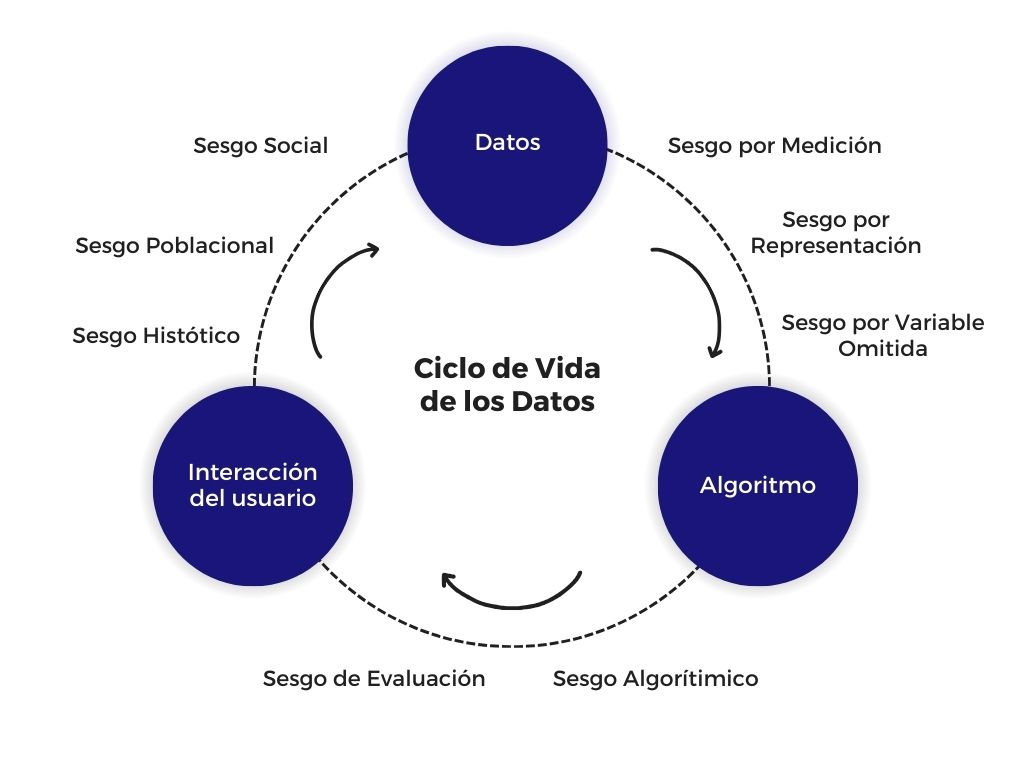
\includegraphics[width=0.7\textwidth]{Graphics/data_cycle.png}
        \end{center}
        \caption{Ejemplos de definiciones de sesgo ubicadas en el ciclo de vida de los datos.}
        \label{fig:cycle}
    \end{figure}
    

    \subsection{Sesgos de los datos al algoritmo}
    
    \begin{itemize}
        \item \textbf{Sesgo por medici\'on}: Surge de como se eligen, utilizan y miden atributos particulares. Un ejemplo de esto se observa 
        en la herramienta de predicci\'on de riesgo de reincidencia COMPAS, donde detenciones anteriores y detenciones de amigos o familiares se utilizaron 
        como variables para medir peligrosidad.
        
        \item \textbf{Sesgo por variable omitida}: Ocurre cuando una o m\'as variables importantes son excluidas del modelo.
        
        \item \textbf{Sesgo por representaci\'on}: Este sesgo se produce de c\'omo se seleccionan las muestras de una poblaci\'on durante el proceso de
        recopilaci\'on de datos. Las muestras no representativas carecen de la diversidad de la poblaci\'on, con subgrupos faltantes y otras anomal\'ias.
    \end{itemize}
    
    \subsection{Sesgos del algoritmo al usuario}

    \begin{itemize}
        \item \textbf{Sesgo algor\'itmico}: Se presenta cuando el sesgo no est\'a presente en los datos de entrada
        y se agrega puramente por el algoritmo. Las elecciones de dise\~no algor\'itmico, como el uso de ciertas funciones de optimizaci\'on, 
        regularizaciones, decisiones en la aplicaci\'on de modelos de regresi\'on en los datos en su totalidad o considerando subgrupos, y el uso
        general de estimadores estad\'isticamente sesgados en algoritmos, todos pueden contribuir a decisiones sesgadas que 
        afectan los resultados de los algoritmos. 
        
        \item \textbf{Sesgo por la interacci\'on del usuario}: El sesgo de interacci\'on del usuario no solo puede observarse en la web, sino que 
        tambi\'en puede ser producido por dos fuentes: la interfaz de usuario y cuando el propio usuario impone su comportamiento sesgado.
        
        \item \textbf{Sesgo de evaluaci\'on}: Ocurre durante la evaluaci\'on del modelo. Esto incluye el uso de m\'etricas
        inapropiadas y desproporcionadas para la evaluaci\'on del modelo. Un ejemplo de esto son las m\'etricas \emph{Adience} y \emph{IJB-A}, 
        que se utilizan en la evaluaci\'on de sistemas de reconocimiento facial que estaban sesgados hacia el color de la piel y el g\'enero.
    \end{itemize}
    
    \subsection{Sesgos del usuario a los datos}

    \begin{itemize}
        \item \textbf{Sesgo hist\'orico}: Es el sesgo y los problemas sociot\'ecnicos ya existentes en el mundo. Puede 
        producirse desde el proceso de generaci\'on de datos, incluso con un muestreo y selecci\'on de caracter\'isticas perfectos.
        
        \item \textbf{Sesgo poblacional}: Surge cuando las estad\'isticas, demograf\'ias y caracter\'isticas 
        de la poblaci\'on de usuarios de la plataforma son diferentes respecto a la poblaci\'on objetivo original, creando datos no
        representativos. Este tipo de sesgo puede surgir de las diferentes demograf\'ias de usuarios en las plataformas sociales, como las
        mujeres que son m\'as propensas a usar \emph{Pinterest}, \emph{Facebook}, \emph{Instagram}, mientras que los hombres 
        son m\'as activos en foros en l\'inea como \emph{Reddit} o \emph{X}.

        \item \textbf{Sesgo social}: Se produce cuando las acciones de otros afectan el juicio de una persona. Un ejemplo de este tipo de 
        sesgo podr\'ia ser un caso en el que la persona quiere otorgar a un elemento una calificaci\'on baja, pero al ser influenciada por otras
        altas, cambia su puntuaci\'on a una calificaci\'on m\'as alta, pensando que quiz\'as esta siendo demasiado severa.
    \end{itemize}

\section{Detecci\'on y mitigaci\'on de sesgos}

Las definiciones de equidad en el contexto de los modelos de aprendizaje autom\'atico conducen 
a un escenario complejo y en constante evoluci\'on. A d\'ia de hoy, no existe una definici\'on \'unica y precisa
de lo que constituye la equidad en este \'ambito. La implementaci\'on de algoritmos en la toma de decisiones automatizada ha desatado 
debates acerca de c\'omo conceptualizar y medir tanto la equidad como la justicia. Estos conceptos no solo involucran consideraciones 
t\'ecnicas, sino que tambi\'en se ven influidos por matices culturales y dilemas \'eticos.

\subsection{Definiciones de equidad}
Las diversas perspectivas sobre la equidad pueden agruparse en dos categor\'ias principales: a nivel de Grupos y a nivel Individual. 
A continuaci\'on se presentan algunas de las definiciones de equidad m\'as relevantes a nivel de grupos:

\begin{itemize}
    \item \textbf{Demographic Parity}: Un algoritmo predictor $\hat{Y}$ satisface \emph{Demographic Parity}
    con respecto a un atributo $A$ con valores en el conjunto $\{0,1\}$ si se cumple $P(\hat{Y} | A = 0) = P(\hat{Y} | A = 1)$. 
    Esto significa que la probabilidad de un resultado positivo debería ser la misma sin importar si el individuo pertenece a
    un grupo protegido~\parencite{fairness_def}.

    \item \textbf{Equal Opportunity}: Un predictor binario $\hat{Y}$ satisface \emph{Equal Opportunity} con 
    respecto a un atributo $A$ y salida $Y$ si $P(\hat{Y} = 1 | A = 1, Y = 1) = P(\hat{Y} = 1 | A = 0, Y = 1)$. Esto significa
    que la probabilidad de que a una persona en la clase positiva le sea asignada un resultado positivo 
    deber\'ia ser igual para miembros tanto de grupos protegidos como no protegidos~\parencite{fairness_def}.

    \item \textbf{Equalized Odds}: Un predictor $\hat{Y}$ satisface \emph{Equalized Odds} con respecto a un atributo
    protegido $A$ y predicci\'on $Y$, si $P(\hat{Y} = 1 | A = 1, Y = y) = P(\hat{Y} = 1 | A = 0, Y = y)$, es decir,
    $\hat{Y}$ y $A$ son independientemente condicionales a $Y$. Esto significa que la probabilidad de que a una persona 
    en la clase positiva le sea asignada correctamente una predicci\'on positiva y la probabilidad de que a una persona en la 
    clase negativa le sea incorrectamente asignada una predicci\'on positiva deber\'ia se la misma para miembros de grupos 
    protegidos y no protegidos~\parencite{fairness_def}.
\end{itemize}

% Otros enfoques relevantes para tratar los sesgos a nivel individual son:

% \begin{itemize}
%     \item \textbf{Fairness Through Awareness}: Individuos con caracter\'isticas similares seg\'un alg\'un criterio 
%     definido deber\'ian obtener resultados parecidos \parencite{fair_awareness}.
%     \item \textbf{Fairness Through Unawareness}: Un algoritmo se considera imparcial cuando no basa sus decisiones en el 
%     atributo protegido \parencite{counterfactual}.
%     \item \textbf{Conterfactual fairness}: Una decisi\'on es considerada imparcial hacia un individuo cuando es la misma
%     tanto en la situaci\'on real como en una situaci\'on hipot\'etica donde el individuo pertenece a otro grupo \parencite{counterfactual}.
% \end{itemize}

\subsection{Mitigaci\'on de sesgos}

Los algoritmos destinados a la mitigaci\'on de sesgos se pueden clasificar esencialmente en m\'etodos de 
pre-procesamiento~\parencite{osti_10182459}, durante el procesamiento~\parencite{ml_in_admissions} y 
post-procesamiento~\parencite{compas}, seg\'un la fase del proceso de aprendizaje en que se realizen. Recientemente, 
han surgido nuevos m\'etodos llamados meta-algoritmos que ofrecen resultados prometedores en diversos escenarios.

Las estrategias de pre-procesamiento buscan la equidad al modificar la representaci\'on de los datos antes de aplicar un modelo de 
aprendizaje autom\'atico. En este proceso se pueden aplicar diversas t\'ecnicas sobre los datos, como eliminar atributos protegidos 
y atributos correlacionados con estos, o bien, modificar las etiquetas de algunos objetos en el \emph{dataset}~\parencite{preproc}. 
Una ventaja de estas t\'ecnicas es que son independientes al modelo. Sin embargo, requieren ajustes de hiperpar\'ametros tanto 
propios como del modelo seleccionado para optimizar su desempe\~no.

Los m\'etodos aplicados durante el procesamiento, modifican los algoritmos de aprendizaje para eliminar la fuente de discriminaci\'on. Esto se 
logra mediante ajustes en la funci\'on objetivo o la aplicaci\'on de restricciones espec\'ificas~\parencite{donini2020empirical,zafar17a}. A pesar de 
que estas t\'ecnicas pueden ser altamente efectivas para la clase espec\'ifica de modelos para la cual fueron dise\~nadas, resulta dif\'icil, e 
incluso en ocasiones imposible, extenderlas a nuevas clases de modelos.

Las t\'ecnicas de post-procesamiento se implementan despu\'es de que el modelo ha sido entrenado, utilizando un conjunto de datos que no haya
participado en dicho proceso. Mediante este procesamiento, las clasificaciones generadas por el modelo se reasignan mediante una funci\'on 
espec\'ifica~\parencite{d_Alessandro_2017}.
Entre las t\'ecnicas de post-procesamiento, se incluyen aquellas que buscan identificar los atributos protegidos que afectan el resultado del 
modelo, y a partir de esto, ajustan la predicci\'on~\parencite{seymour2018bias}. La principal limitaci\'on radica en que ajustar la predicci\'on 
en esta fase es inherentemente sub\'optimo y puede resultar en un peor equilibrio entre eficacia y equidad.

Por \'ultimo, cabe destacar la relevancia de los meta-algoritmos, una categor\'ia de m\'etodos recientemente propuesta para problemas de 
mitigaci\'on de sesgos. Estos simplifican dicha tarea a una serie de problemas de clasificaci\'on, cada uno con 
un costo asociado a sus errores de predicci\'on~\parencite{agarwal2018reductions, agarwal2019fair}.
A diferencia de los m\'etodos que operan durante el procesamiento, los meta-algoritmos son independientes al tipo de modelo utilizado en el 
clasificador base, solo dependen de la capacidad de este para ser reentrenado repetidamente. Las soluciones a estos problemas suelen generar
un clasificador randomizado.

\subsection{Anotaci\'on autom\'atica de atributos protegidos}
La anotaci\'on autom\'atica de atributos protegidos es una t\'ecnica que demuestra ser prometedora para asistir en la detecci\'on y 
mitigaci\'on de sesgos~\parencite{soumah2023radar,dinan2020multidimensional,10.1007/978-3-031-35320-8_39,6906255,Rajendra_2021}. 
Esta t\'ecnica involucra el uso de modelos de aprendizaje autom\'atico para predecir la pertenencia de los datos a grupos protegidos, 
como g\'enero, raza, orientaci\'on sexual, entre otros. 

Los modelos autom\'aticos entrenados para la detecci\'on de atributos protegidos pueden incorporarse en el desarrollo de t\'ecnicas
de mitigaci\'on de sesgos de varias maneras:
\begin{itemize}
    \item Permitiendo una detecci\'on m\'as amplia de sesgos en conjuntos de datos a gran escala.
    \item Proporcionando atributos protegidos predichos que pueden utilizarse en t\'ecnicas basadas en 
    la equidad de grupos.
    \item Generando conjuntos de datos sint\'eticos con atributos protegidos para el entrenamiento y evaluaci\'on de 
    modelos.
    \item Haciendo posible el an\'alisis de sesgos en casos donde la recopilaci\'on manual de los atributos protegidos
    puede ser dif\'icil, invasiva o poco \'etica.
\end{itemize}

Sin embargo, la precisi\'on de los modelos autom\'aticos est\'a limitada por la calidad de los datos de entrenamiento. Por ello, es 
recomendable complementar estas predicciones con revisiones manuales por parte de expertos.
 
\section{Datasets en el an\'alisis de sesgos}
    % \begin{itemize}
    %     \item empezar hablando de como los datasets ayudan a desarrollar y evaluar tecnicas de evaluacion y mitigacion de sesgos
    %     \item luego mencionar y decir algo de los datasets clasicos con datos tabulares
    %     \item luego empezar a hablar de datasets con datos no tabulares en general y decir que hay pocos y que son dificiles de conseguir 
    %     \item hablar luego de datasets interesantes que se pueden utilizar para esto (los estudiados)
    %     \item Decir algunos datos interesantes de cada uno
    % \end{itemize}

    Los \emph{datasets} con atributos protegidos anotados juegan un papel fundamental en el desarrollo y evaluaci\'on de t\'ecnicas destinadas 
    a mitigar sesgos. Estos proporcionan la informaci\'on necesaria para la identificaci\'on, cuantificaci\'on y abordaje de sesgos, 
    permitiendo as\'i la creaci\'on y validaci\'on de t\'ecnicas dirigidas a mejorar la equidad y justicia en modelos de aprendizaje 
    autom\'atico. 
    Un \emph{dataset} representativo y diverso es esencial para el desarrollo de estrategias eficaces que mitiguen sesgos en diversas aplicaciones. 
    Los \emph{datasets} pueden categorizarse en dos grupos seg\'un la configuraci\'on de sus datos: 
    aquellos con datos tabulares\footnote{Est\'a organizado en forma de tabla, donde los datos se presentan en filas y columnas. Cada fila 
    representa una entrada individual, y cada columna es una caracter\'istica espec\'ifica con valores num\'ericos, categ\'oricos u otros.} 
    y aquellos con datos no tabulares\footnote{No sigue la estructura de una tabla tradicional, puede tener informaci\'on m\'as compleja, como 
    texto, im\'agenes o audio}.
    
    \subsection{Datasets con datos tabulares}
    Entre los \emph{datasets} con estructura tabular m\'as relevantes utilizados para el an\'alisis y la evaluaci\'on de modelos destinados 
    a la mitigaci\'on de sesgos~\parencite{calmon2017optimized,wang2023mitigating,compas}, se incluyen:

    %#TODO deberia annadir una tabla tambien de tabulares?????
    \begin{itemize}
        \item \textbf{Adult}: Tambi\'en conocido como \emph{Census Income}, este \emph{dataset} contiene $48\,842$ registros de 
        datos sobre el censo de 1994 en Estados Unidos. Incluye $14$ atributos, como edad, educaci\'on, estado civil,
        ocupaci\'on, raza, g\'enero, pa\'is de origen, horas de trabajo por semana, entre otros. Adem\'as, para cada 
        persona indica si sus ingresos son mayores o menores a $50$ mil d\'olares anuales.
        \item \textbf{Compas}: Este \emph{dataset} contiene $18\,610$ registros de los acusados del condado de Broward, Florida,
        indicando sus tiempos en la c\'arcel y prisi\'on, datos demogr\'aficos, antecedentes penales y puntuaciones 
        de riesgo, desde 2013 hasta 2014.
        \item \textbf{German Credit}: El \emph{dataset} \emph{German Credit} contiene registros del estado financiero de $1\,000$ individuos,
        que incluye atributos como g\'enero, puntaje crediticio, monto del cr\'edito, estado de vivienda, entre otros. Adem\'as cada 
        persona es clasificada como un riesgo crediticio bueno o malo, seg\'un el conjunto de atributos.
        \item \textbf{Communities and Crime}: Este \emph{dataset} recopila informaci\'on de diversas comunidades en Estados Unidos, 
        relacionada con varios factores que pueden influir significativamente en algunos delitos comunes, como robos, asesinatos o 
        violaciones. Los datos incluyen informaci\'on sobre delitos, obtenida de la encuesta \emph{LEMAS} de Estados Unidos en 1990 y 
        del \emph{Informe Unificado de Delitos del FBI} en 1995. Adem\'as, se incluyen datos demogr\'aficos y socioecon\'omicos del 
        censo de 1990.

    \end{itemize}

    \subsection{Datasets con datos no tabulares}
    Los \emph{datasets} con datos no tabulares y atributos protegidos anotados, como im\'agenes, audio, texto y otros formatos complejos, 
    son considerablemente menos comunes que los \emph{datasets} con datos tabulares. Esto se debe a la complejidad y el costo asociado a la 
    recopilaci\'on, etiquetado y mantenimiento de datos no tabulares.

    Mientras que los datos tabulares son adecuados para problemas estructurados, los datos no tabulares permiten abordar tareas m\'as diversas, 
    como reconocimiento de im\'agenes, procesamiento de lenguaje natural, an\'alisis de audio y textos. Esto los convierte en un recurso muy importante
    para el desarrollo y evaluaci\'on de t\'ecnicas de mitigaci\'on de sesgos en estos escenarios. En la Tabla~\ref{table:datasets} 
    se presentan algunos ejemplos relevantes de \emph{datasets} con datos no tabulares y atributos protegidos anotados de inter\'es para el 
    an\'alisis de sesgos.

    \begin{table}[htpb]
        \centering
        \resizebox{\textwidth}{!}{
            \begin{tabular}{lp{0.34\textwidth}p{0.34\textwidth}p{0.34\textwidth}}
            \toprule
            \toprule
                \textbf{Dataset}     & \textbf{Twitter Gender}                          & \textbf{Md Gender Funpedia}                         & \textbf{Bias in Toxicity}       \\
                \toprule
                \toprule
                Tipo de datos        & Texto                                            & Texto                                               & Texto                           \\
                \midrule
                Atributos destacados & Existencia o no de sesgo                         & G\'enero                                            & G\'enero, raza, religi\'on, orientaci\'on sexual y discapacidad  \\
                \midrule
                Idioma               & Espa\~nol                                        & Ingl\'es                                            & Ingl\'es                        \\
                \midrule
                Tipo de Lenguaje     & Chitchat                                         & Formal                                              & Informal                        \\
                \midrule
                Tama\~no             & $1.9$K                                           & $29.8$K                                             & $1.9$M                          \\
                \midrule
                Tipo de Anot.        & Desconocido                                      & Preanotado autom\'aticamente y revisado manualmente & Manual                          \\
                \midrule
                Fuente de datos      & P\'aginas web que abordan los sesgos de g\'enero & Wikipedia                                           & Plataforma Civil Comments       \\
                \toprule
                \toprule
                \textbf{Dataset}     & \textbf{Fair Face}                               & \textbf{UTKFace}                                    & \textbf{MTGenEval}              \\
                \toprule
                \toprule
                Tipo de datos        & Im\'agenes                                       & Im\'agenes                                          & Texto                           \\
                \midrule
                Atributos destacados & G\'enero, raza y edad                            & G\'enero, raza y edad                               & G\'enero                        \\
                \midrule
                Idioma               & -                                                & -                                                   & Ingl\'es, espa\~nol, ar\'abico, franc\'es, alem\'an, hind\'u, italiano, portugu\'es y ruso\\
                \midrule
                Tipo de Lenguaje     & -                                                & -                                                   & Informal                        \\
                \midrule
                Tama\~no             & $108$K                                           & $20$K                                               & $4$K                              \\
                \midrule
                Tipo de Anot.        & Manual                                           & Semi-autom\'atica                                   & Manual                          \\
                \midrule
                Fuente de datos      &  Dataset YFCC-100M Flickr                        & Datasets MORPH y CACD y web                         & Wikipedia                       \\
                \bottomrule
                \bottomrule
            \end{tabular}}
        \caption{Resumen de datasets con datos no tabulares}
        \label{table:datasets}
    \end{table}
    
    El \emph{dataset} \emph{Twitter Gender}\footnote{\url{https://www.kaggle.com/datasets/kevinmorgado/gender-bias-spanish}} est\'a conformado por 
    \emph{tweets} en espa\~nol, etiquetados con la categor\'ia de sesgado o no sesgado. Inicialmente el \emph{dataset} no est\'a dividido en subconjuntos de 
    entrenamiento y prueba.

    El \emph{dataset} \emph{Md Gender Funpedia}\footnote{\url{https://huggingface.co/datasets/md_gender_bias/viewer/funpedia}} contiene oraciones de 
    Wikipedia, reformuladas de una manera m\'as conversacional~\parencite{dinan2020multidimensional}. Se conservan \'unicamente las oraciones 
    vinculadas a biograf\'ias. Cada oraci\'on est\'a etiquetada con el g\'enero de quien se habla. Adem\'as est\'a dividido en subconjuntos de 
    entrenamiento, prueba y validaci\'on.

    El \emph{dataset} \emph{Bias in Toxicity}\footnote{\url{https://www.kaggle.com/competitions/jigsaw-unintended-bias-in-toxicity-classification}}
    est\'a formado por comentarios de individuos, con gran cantidad de atributos protegidos anotados. Tambi\'en se 
    indica el nivel de toxicidad y toxicidad severa de cada comentario. Cada atributo es un valor entre $0$ y $1$ que indica la probabilidad de 
    que el comentario pertenezca a la clase correspondiente. Este \emph{dataset} aporta tambi\'en los subconjuntos de entrenamiento y prueba, adem\'as 
    de otros subconjuntos relacionados con la anotaci\'on del mismo.  

    El \emph{dataset} \emph{Fair Face}\footnote{\url{https://github.com/joojs/fairface}} contiene im\'agenes de rostros, con los atributos edad, 
    g\'enero y raza anotados. Est\'a balanceado respecto a la raza~\parencite{karkkainenfairface} e incluye los subconjuntos de entrenamiento y 
    validaci\'on.

    El \emph{dataset} \emph{UTKFace}\footnote{\url{https://www.kaggle.com/datasets/jangedoo/utkface-new}} est\'a formado por im\'agenes de rostros, que 
    presentan una gran variaci\'on en la pose, expresi\'on facial, iluminaci\'on, oclusi\'on y resoluci\'on~\parencite{zhang2017age}. 
    Tiene anotados los atributos protegidos edad, g\'enero y raza. Presenta desbalance respecto a estos atributos, con predominio de la raza 
    blanca y el g\'enero masculino. Inicialmente no se incluyen los subconjuntos de entrenamiento y prueba.

    El \emph{dataset} \emph{MTGenEval}\footnote{\url{https://github.com/amazon-science/machine-translation-gender-eval}} contiene oraciones en 
    diferentes idiomas que se traducen mejor considerando el contexto inter-sentencial\footnote{Se refiere a la informaci\'on que se puede 
    inferir de la oraci\'on} y oraciones que se traducen mejor cuando se cambia una palabra o frase espec\'ifica. Incluye atributos protegidos 
    relacionados con el g\'enero, ejemplos de oraciones estereotipadas y antiestereotipadas. Se utiliza para entrenar y evaluar modelos de 
    traducci\'on autom\'atica, prestando especial atenci\'on a la equidad de g\'enero en dichas traducciones~\parencite{Currey2022}.

\section{Discusi\'on}

Los \emph{datasets} presentados anteriormente constituyen un recurso valioso para apoyar el estudio, desarrollo y evaluaci\'on de t\'ecnicas de 
mitigaci\'on de sesgos en modelos de aprendizaje autom\'atico. Sin embargo, la principal limitante de estos es que ninguno ofrece 
informaci\'on sobre decisiones tomadas sobre los sujetos, como la decisi\'on de otorgar un pr\'estamo o la de contratar a una persona.

Esta limitante es significativa porque impide una evaluaci\'on completa sobre si las decisiones tomadas por los algoritmos basados 
en los datos son sesgadas o no. Por ejemplo, si un algoritmo se utiliza para tomar decisiones de contrataci\'on bas\'andose en datos
sobre solicitantes de empleo, incluyendo su g\'enero y raza, ser\'ia \'util conocer si a cada solicitante le fue ofrecido 
un trabajo o no. Esta informaci\'on permitir\'ia evaluar si el algoritmo se inclina a ofrecer trabajos a personas con cierto g\'enero o raza
por encima de otras.

Por lo tanto, en el contexto de esta tesis, que tiene como objetivo el dise\~no y evaluaci\'on de un corpus de estructura no tabular
con atributos protegidos anotados, es importante considerar la inclusi\'on de informaci\'on sobre las decisiones tomadas sobre los sujetos.
El corpus de rese\~nas de pel\'iculas \emph{IMDb}\footnote{\url{https://www.kaggle.com/datasets/mantri7/imdb-movie-reviews-dataset}}
cumple con esta restricci\'on, ya que incluye el sentimiento presente en cada rese\~na, que puede considerarse como una decisi\'on de 
recomendaci\'on. Adem\'as si se realiza la anotaci\'on manual de los atributos g\'enero y raza para cada texto, se obtendr\'ia un corpus
que cumple con todas las restricciones planteadas en los Objetivos Generales.